\chapter{Rationale for statewide modeling}\label{sec:rationale-for-statewide-modeling}

Statewide modeling is undertaken to inform a wide variety of policy analysis, planning, investment, and programming activities. The range of reported uses is described in this chapter. It is divided into three parts. The first part describes the primary uses of statewide models, with an emphasis on how they differ from metropolitan (or urban) models. The evaluation of the impacts of State Long-Range Transportation Plans (LRTP) is perhaps the most common application of statewide models. The second part describes scenario analysis conducted with statewide models, and provides insights from the survey on the types of scenarios predominantly analyzed. Finally, the third part deals with performance measures in statewide modeling.

\section{Motivations for statewide modeling}

Statewide models are used to analyze the impact of policies and trends that are implemented or addressed by state governments, but not captured with urban or national models. This includes several travel markets not commonly included or underrepresented in urban models:

\begin{itemize}
\item
Foremost, statewide models capture travel occurring in areas outside of major metropolitan areas. Smaller MPOs and agencies outside of them often do not operate their own transportation models, yet there is a need to analyze transportation planning in these areas as well. In practice, state DOTs commonly fulfill this role using statewide models.
\item
Metropolitan transportation models cannot capture travel between MPOs. For example, the three MPOs in Arizona --- the Maricopa Association of Governments (MAG) in Phoenix, Sun Corridor Metropolitan Planning Organization in Pinal County, and Pima Association of Governments (PAG) in Tucson --- share borders and have substantial travel between them. However, their models focus on travel within each area. A statewide model is used to fully represent travel demand in the corridor between Phoenix and Tucson. Similar examples include travel between the San Diego and Los Angeles areas, or between Baltimore and Washington, D.C. Statewide models have been developed to capture travel between these areas.
\item
Long-distance travel is of concern in statewide models. MPO models commonly represent travel with origins or destinations outside their MPO area as external trips. They enter or leave at external stations, which do not distinguish between final destinations two miles versus two thousand miles away. Both ends of such trips are often explicitly represented in statewide models, which is necessary given the size of study areas for most states. There is no universal definition of long-distance travel. The National Household Travel Survey (NHTS) defines long-distance travel as trips with 50 miles or more, and the older American Travel Survey (ATS) as 100 miles or more. Long-distance travel behavior differs substantially from short-distance travel, which is why most statewide models explicitly distinguish between them. The former is infrequent, with different destinations (more concentrated in city centers of major metropolitan areas), a mix of modes different from local travel, different hours during the day (less focused on morning and evening peak hours), and different path choices. Long-distance travelers have traditionally tended to stay on highways and major arterials, for they are not as familiar with local streets. However, this tendency is reduced by the use of navigation systems.
\item
Freight is a key market represented in most statewide models. Twenty of the 34 states that operate or are developing statewide models include short-distance truck flows, and 26 model long-distance truck flows explicitly (59 and 76 percent, respectively). Most urban models capture truck flows as well, but many of them travel outside of the modeled area, necessitating their representation in statewide models. Freight moving by rail, water, and air are irrelevant in urban models, apart from where they transfer to trucks. With larger study areas for states, these modes become more important. Accordingly, 13 states (or 38 percent) have implemented explicit freight mode choice models.
\item
Statewide models can provide external traffic volumes for urban models. In many cases, urban models prefer to use traffic counts at external stations and distribute those volumes between internal zones and other external stations using gravity models. Using a statewide model for this purpose, however, offers two significant advantages. First, the statewide model explicitly distinguishes between origins and destinations that are internal to the MPO region from those that are external. This lead to a better distinction between through, internal-to-external, and external-to-internal trips, rather than relying upon under-specified gravity models to make this distinction. Secondly, using statewide model forecasts for urban models allows accounting for the impact of scenarios that may affect traffic flows outside the MPO area. For instance, a major highway project within an MPO region may affect the routing of long-distance trips with origins and destinations outside of it. Running this scenario in the statewide model first to generate updated external volumes, and then with the MPO model using these revised external volumes, will create consistency between long and short-distance travel.
\end{itemize}

Some states also develop ``officially sanctioned'' datasets and forecasts using statewide models. Consistent zonal socioeconomic datasets and --- even more challenging --- forecasts provide data that states can work with and refer to. Traffic counts sometimes are mapped to statewide model networks, providing a common reference system used across agencies within a state. In the same vein, statewide models may also be tools that facilitate cooperation between different agencies.

%\protect\hypertarget{h.ra3igdrh8psb}{}{}
At the same time, it is also important to recognize what statewide models are not well suited for. There are no known domain reasons why statewide models cannot be used for certain analyses. Rather, insufficient spatial and temporal resolution in statewide models may be an impediment to analyzing scenarios that are more commonly addressed using urban models. For example, most statewide models are too coarse to adequately represent non-motorized travel (i.e., walk or bike). The impact of transit-oriented development is another example that requires higher spatial resolution around transit stations than commonly found in statewide models. Likewise, impacts of very small projects, such as a new highway ramp, tend to be overlooked by statewide models for lack of spatial resolution. Statewide models also tend to be less capable of representing detailed and complex urban transit systems, even though the Google Transit Feed Data (discussed further in Chapter \ref{sec:emerging-methods-opportunities}) may overcome this limitation for statewide models to some degree.

\section{Scenario analysis}\label{sec:scenario-analysis}

Statewide and megaregional models are built to test scenarios to advise policy-makers. Such scenarios may include:

\begin{itemize}
\item
\emph{Infrastructure scenarios} test the impact of new infrastructure, such as the extension of a road, the implementation of a new transit line, or the development of additional housing in a specific location. These scenarios refer to changes in the built environment. They may also include scenarios of disinvestment, such as abandoning or curtailing infrastructure maintenance.
\item
\emph{Policy scenarios} test the impact of alternative policies to handle transport, such as raising tolls on a highway link, prohibiting trucks from using selected roads, or increasing the frequency of transit service. Policy scenarios test alternative regulations that could be actively implemented by a jurisdiction without significantly changing the built environment.
\item
\emph{Global scenarios} test the impact of uncertain future developments, such as increased immigration, rising energy prices or widespread adaptation of autonomous vehicles. Changing conditions tested in global scenarios usually cannot be influenced by local policy makers, but are rather given as an exogenous constraint the region must adopt. These scenarios are commonly used to understand the range of impact, such as testing different levels of them on congestion (Figure \ref{fig:immigration-vs-congestion}).
\end{itemize}

\begin{figure}
\centering
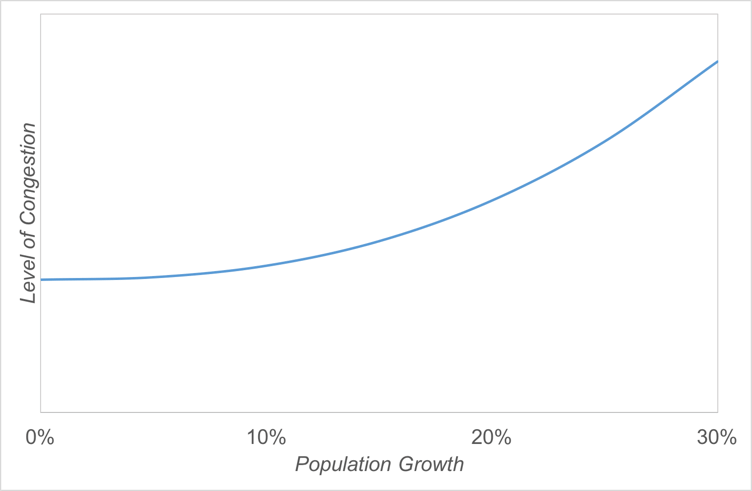
\includegraphics[scale=0.4]{graphics/03-immigration-vs-congestion}
\caption{Hypothetical relationship between immigration and level of congestion}
\label{fig:immigration-vs-congestion}
\end{figure}

Often, models are developed with specific applications in mind. For example, it was imperative that agricultural flows, which change by season, were represented realistically in Idaho's Statewide Model. The Maryland Statewide Model was built predominantly to test highway scenarios that apply to areas outside of the Baltimore and Washington metropolitan areas. Sensitivity to changes in zoning was a key design feature of Oregon's Statewide Model.

The survey asked explicitly for what kind of scenarios were evaluated using statewide models. Respondents could select more than one answer, which is why the total of all responses is much larger than the number of states that operate statewide models. A summary of the common scenarios is shown in Figure \ref{fig:typical-scenarios}. Light bars indicate scenarios described as most important.

\begin{figure}  % 4
\centering
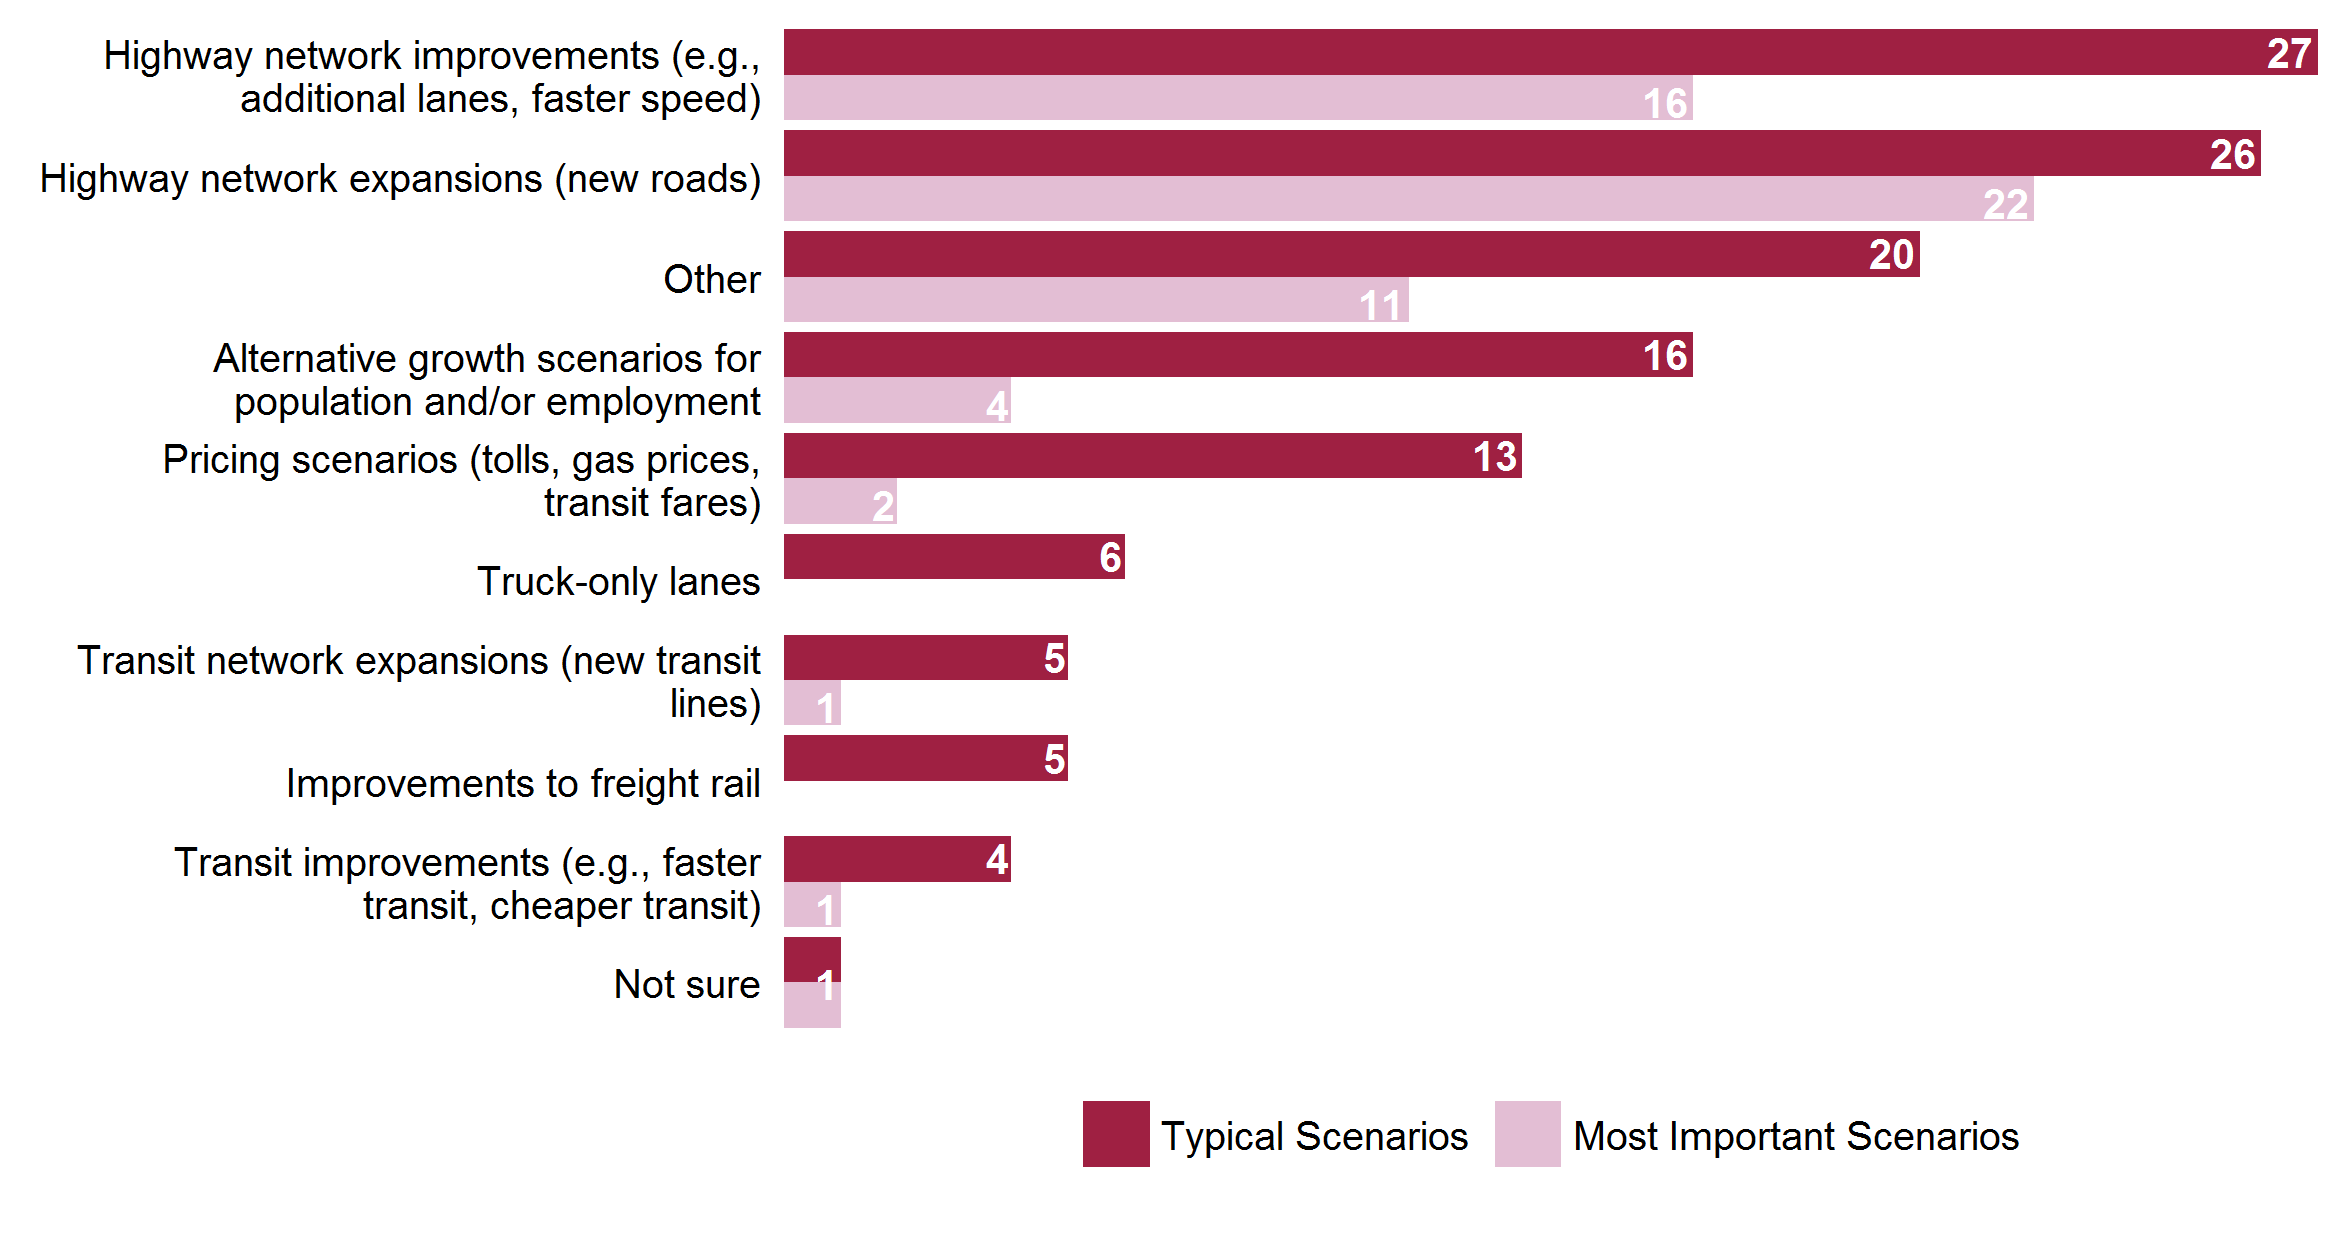
\includegraphics[width=6in]{graphics/04-typical-scenarios-tested}
\caption[Typical scenarios tested with statewide models]{Typical scenarios tested with statewide models (multiple answers allowed)}
\label{fig:typical-scenarios}
\end{figure}

By far the most common application of statewide models (27 respondents, or 79 percent) involved testing of highway network improvements, including additional lanes, change of speed and similar network enhancements. Testing the impacts of network additions (i.e., the construction of entirely new roads) was a close second. This was not surprising, as state and local governments together spend six times as much on highways as they spend on transit \citep{usdot14}. The next most important scenario type was global scenario testing of the impact of alternative population growth rates. Sixteen of the 34 states that conduct statewide modeling (47 percent) reported using statewide models to test alternative growth forecasts. This finding underlines the large uncertainties associated with population and employment forecasts. States can assess the viability and resilience of their transportation system under a variety of alternative futures.

Pricing scenarios (including tolls, gas price increases and transit fares) were tested by 13 states (or 38 percent of states that conduct statewide modeling). The interest in and necessity of testing alternative pricing structures is on the rise, as lack of alternative forms of funding pushes transportation agencies to charge for the use of infrastructure \citep{perez12}. As such, it is rather surprising that only slightly more than a third of states with models test pricing scenarios. A possible explanation might be that pricing strategies are more predominant in local jurisdictions. Tolled highway infrastructure, such as Interstate Turnpikes, tend to be administered by commissions that are independent of state DOTs, often operating separate models.

A few states listed ``Other'' scenarios relevant to them. Four states (Kentucky, Maine, Michigan and Vermont) specifically added that they use the statewide model to analyze road closure for highway construction and maintenance. Texas and Utah pointed out that they use their statewide models to analyze freight. Indiana and Nebraska use the statewide model for subarea analyses and select link analyses, which allows identifying traffic volumes and trip origin and destinations in a selected part of the state or on individual links. Oregon also used their statewide model to analyze the impact of weight-restricted bridges, seismic impacts, and economic impacts of various levels of investment. Massachusetts also used their model for air quality conformity analysis. Florida conducts evacuation analyses. Five case studies are described in more detail in Chapter \ref{sec:case-studies}, with a special focus on the type of applications these models are used for.

\section{Performance measures}

Assessing changes in performance measures under different scenarios is an important use of state\-wide models. Such measures evaluate how efficient a transport system operates in terms of consistent metrics, such as reliability and travel time delay and variability. Even though not written specifically for modelers, a good overview of performance measures commonly used by transportation planning agencies is provided in NCHRP Report 618 \citep{cambridge08}. Statewide models are commonly expected to provide similar outputs to ensure that the models can be used to evaluate performance measures under various scenarios. Performance measures are often categorized by four dimensions:

\begin{itemize}
\item Duration, or how many hours the delay on the network lasts
\item Extent, or how many people or vehicles are affected
\item Intensity, or by how much travel time is delayed, and
\item Variability, describing whether the congestion pattern is similar every day (such as expected peak hour congestion) or irregular (such as delays caused by incidents)
\end{itemize}

Travel demand models are reasonably strong at predicting the second and third dimensions, but inherently bad at assessing the first and last issues. Some statewide models only represent daily total traffic, making it impossible to assess the duration of congestion. Several models distinguish four time-of-day periods, which allows only coarse evaluation of congestion duration. Runtimes of the assignment step tend to be long. Therefore, all statewide models analyzed in this report distinguished four time-of-day periods at most, except for Colorado, where they plan to work with seven to 10 periods. The representation of variability is almost non-existent in statewide models. Such models typically represent an average day rather than the observed variability from one day to the next.

Performance measures that are typically used in conjunction with transportation models commonly include:

\begin{itemize}
\item Travel time in minutes (vehicle-hours traveled)
\item Travel delay in minutes (vehicle-hours delay)
\item Travel distance in miles (vehicle-miles traveled)
\item Travel distance diversion in miles (actual traveled distance under congested conditions minus shortest paths in free-flow travel environments)
\item Average speed
\item Vehicle or traveler throughput
\item Percent of congested segments (miles of network links under congestion divided by total miles of network length)
\item Equity analysis, such as whether certain income groups benefit more from a certain investment than others
\item Gaseous emissions (such as CO\textsubscript{2}, PM, NO\textsubscript{x}) or noise generated, if an environmental impact capability is implemented
\item Economic benefits of investments (often measured as changes in gross domestic product), if economic impact modeling is implemented
\end{itemize}

\noindent Such measures can be expressed as either per traveler, per vehicle, or as a system-wide total.

The Moving Ahead for Progress in the 21st Century Act (MAP-21) required the Secretary, in consultation with States, MPOs and other stakeholders, to establish performance measures in the areas of:

\begin{enumerate}
\item Pavement condition on the Interstate System and the remainder of the National Highway System (NHS)
\item Performance of the Interstate System and the remainder of the NHS
\item Bridge condition on the NHS
\item Fatalities and serious injuries --- both number and rate per vehicle mile traveled --- on all public roads
\item Traffic congestion
\item On-road mobile source emissions
\item Freight movement on the Interstate System
\end{enumerate}

States were required to set performance targets in support of those measures. While MAP-21 did not explicitly call for transportation modeling, statewide models were routinely used to assess at least items 2, 5, 6, and 7. It is thought that these measures will remain important in the more recent Fixing America's Surface Transportation (FAST) Act of 2015.